\documentclass[red, aspectratio=169, xcolor=dvipsnames]{beamer} 
%Definições de tema
\setbeamertemplate{blocks}[rounded][shadow=false]
\usetheme{Madrid}
\setbeamertemplate{items}[square]
\setbeamertemplate{caption}[numbered]
\usecolortheme{beaver}
\setbeamercolor{frametitle}{bg=white!10!white}

\usefonttheme{professionalfonts}
\setbeamertemplate{itemize item}{\color[rgb]{0.8,0,0}$\blacksquare$}
\setbeamertemplate{itemize subitem}{\color[rgb]{0.8,0,0}$\blacksquare$}
\setbeamertemplate{itemize subsubitem}{\color[rgb]{0.8,0,0}$\blacksquare$}

%Definições de seção
\setcounter{secnumdepth}{3}
\setcounter{tocdepth}{2}


\usepackage{textcomp}
\usepackage{xkeyval}
\usepackage{todonotes}
\presetkeys{todonotes}{inline}{}

\usepackage{tikzsymbols}
\usepackage{helvet}
\renewcommand{\familydefault}{\sfdefault}
\usepackage{float}
\usepackage[brazil]{babel}
\usepackage[utf8]{inputenc}
\usepackage{graphicx}
\usepackage{url}
\usepackage{subfigure}
\usepackage{mathtools} % setas com texto
\usepackage{multicol}
\usepackage{listings}
\usepackage{scalefnt}
\usepackage{ragged2e}
\usepackage{etoolbox, verbatim}

% Listing
\lstset{
	numbers=left,
	stepnumber=1,
	numbersep=5pt,
	numberstyle=\small\color{black},
	basicstyle= \scriptsize,
%	keywordstyle=\color{black},
%	commentstyle=\color{black},
%	stringstyle=\color{black},
	tabsize=2
}

\let\olditem=\item%
\renewcommand{\item}{\olditem \justifying}

\title[Arquitetura de Computadores - RISC-V]{\textbf{Arquitetura de Computadores}\\\textit{Reduced Instruction Set Computer: RISC-V}}
\author[\textit{rodolfolabiapari@decom.ufop.br}]{Rodolfo Labiapari Mansur Guimarães}
\institute[IFMG]{\begin{figure}
			\centering
			
\includegraphics[width=0.1\textwidth]{img/ufop.jpg}
		\end{figure}}
\institute[UFOP]{
	\textit{rodolfolabiapari@decom.ufop.br} \\
	Lattes: \url{http://goo.gl/MZv4Dc} \\
	Departamento de Computação -- Universidade Federal de Ouro Preto \\
	Ouro Preto - MG -- Brasil }

\date{Última Atualização: \today}

\begin{document}


\frame{\titlepage}

\AtBeginSection[]
{
	\begin{frame}
	\frametitle{Sumário}
	\tableofcontents[]
	\end{frame}
}

\AtBeginSubsection[]
{
	\begin{frame}
	\frametitle{Sumário}
	\tableofcontents[
    currentsection,
    currentsubsection,
    hideothersubsections,
    %sectionstyle=show/hiden,
    subsectionstyle=show/shaded, ]
	\end{frame}
}


%\usebackgroundtemplate{
\includegraphics[trim=0cm 0cm 10cm 0cm, width=0.03\textwidth]{img/ufop.jpg}}

\section{Introdução}
\begin{frame}{Introdução ao RISC-V}
	\begin{block}{RISC-V}
		Um moderno e de alta qualidade \textit{Conjunto de Instruções para Computador de Propósito Geral}, o ISA RISC-V.
	\end{block}
	\begin{itemize}
		\setlength{\itemsep}{1.5em}

		\item RISC-V é um ISA\footnote{\textit{Instruction-Set Archtecture.}} \textit{open-source} desenvolvido por 
		\begin{itemize}
			\item \textbf{Profissionais}, \textbf{Professores} e \textbf{Voluntários Entusiastas} no ramo de Arquiteturas de Computadores;
		\end{itemize}
	
		\begin{itemize}
			\item Pessoas que possuem \textbf{experiência} em várias especialidades
			\begin{itemize}
				\item Eletrônica Digital, Compiladores, Sistemas Operacionais, Microprocessadores, entre outras como simulação e validação dos design do projeto.
			\end{itemize}
		
			\item Foi desenvolvido com base em uma série de outros projetos acadêmicos de \textit{design} de computadores.
		\end{itemize}

	\end{itemize}
\end{frame}


\begin{frame}{Introdução ao RISC-V}
	\begin{itemize}
		\setlength{\itemsep}{1em}
		\item Foi produzido pela \textit{Computer Science Division} na Universidade da Califórnia, Berkeley.

		\item É um conjunto de instruções
		\begin{itemize}
			\item \textbf{Limpo};
			\item \textbf{Modular}
			\item Inteiros com bases em 32, 64 e 128 bits e;
			\item Várias opções de \textbf{extensão de instruções} como ponto-flutuante, multiplicadores, etc.
		\end{itemize}
	\end{itemize}
\end{frame}


\begin{frame}{Introdução ao RISC-V}
	\begin{itemize}
		\setlength{\itemsep}{1em}
		
		\item Cada empresa/usuário espera que os \textit{designers} considerem a \textbf{performance} e também a \textbf{eficiência energética} ao projetar um processador novo processador. Mas isso é um \textit{trade-off}
		\begin{itemize}
			\item Em contrapartida, RISC-V é um projeto cujas instruções são de fácil implementação comparado a outras alternativas existentes no mercado;
			\item E mesmo sendo um projeto novo, possui grande aceitação na indústria de semicondutores.
		\end{itemize}
	\end{itemize}

	\begin{block}{Meta}
		 Criar um conjunto de instruções `universal', que é livre e aberto para todos os usuários, provendo tudo que é necessário para suportar perfeitamente qualquer projeto comercial.
	\end{block}
\end{frame}

\begin{frame}{Introdução ao RISC-V}{Comparação com outros ISAs}
	\begin{itemize}
		\setlength{\itemsep}{1em}
		
		\item Não é o primeiro projeto \textit{open-souce}
		\begin{itemize}
			\item É modelado para ser útil desde \textbf{projetos embarcados de pequeno porte} até \textbf{servidores}, \textbf{celulares \textit{high-end}}.
			
			\item Incluindo fazer \textit{design}, fabricar e vender os chips e \textit{software} RISC-V.
		\end{itemize}

		\item O ISA RISC-V tem sido desenvolvido com o intuito de ser 
		\begin{itemize}
			\item Pequeno, rápido e de gasto mínimo de energia em implementações em especificações RISC existente hoje
			
			\item Sem sobrecarregar outras partes do seu sistema (\textit{trade-off}).
		\end{itemize}
	\end{itemize}
\end{frame}


\begin{frame}{Introdução ao RISC-V}{Comparação com outros ISAs}
	\begin{itemize}
		\setlength{\itemsep}{1em}
		
		\item Embora alguns processadores disponíveis hoje no mercado sejam amplamente utilizados, eles \textbf{são complexos} e difícil de ser utilizado para experimentação e uso acadêmico.
		
		\item Difere da maioria dos ISA pois, chips da ARM e MIPS Technologies necessitam de licença para uso de suas patentes
		\begin{itemize}
			\item Também requerem acordos de confidencialidade para uso de seus documentos que citam as vantagens de seus \textit{design} e conjunto de instruções.
		\end{itemize}
	
		\item Sua arquitetura é mais fácil de ser implementada do que um ARM, por exemplo:
		\begin{itemize}
			\setlength{\itemsep}{0.5em}
			\item Pela sua simplicidade em:
			\begin{itemize}
				\item Decodificar códigos e modos de endereçamento.
			\end{itemize}
			\item Omite instruções complexas;
			\item Tudo isso com \textbf{metade} do tamanho de projeto de um ARM \textit{core}.
		\end{itemize}
	\end{itemize}
\end{frame}

\begin{frame}{De Projeto Acadêmico à Oracle e Google}
	\begin{itemize}
		\setlength{\itemsep}{1.5em}
		\item Iniciado em 2010;
		
		\item Disponibilizado em 2015;
		
		\item E já é utilizado pela Mellanox, Oracle e Google, além de grandes centros acadêmicos.
		
		\item Por ser \textit{open-source}, vários projetos funcionais online já estão disponíveis, usufruindo da permissão de licença BSD
		\begin{itemize}
			\item Um exemplo é o escalar de 5 estágios chamado RISC-V Rocket\footnote{Disponível em: \url{https://github.com/ucb-bar/rocket}} em Scala e para sintetização em chips\footnote{Disponível em: \url{https://github.com/ucb-bar/rocket-chip}}.
		\end{itemize}
	
		\item É considerado como a técnica mais \textbf{promissora} em flexibilidade de extensões customizadas combinado com arquitetura de propósito geral.
	\end{itemize}
\end{frame}


\subsection{Exemplificação}
\begin{frame}{Exemplificação}
	Consideremos um \textit{smartphone} moderno \textit{high-end}.
	\begin{itemize}		
		\setlength{\itemsep}{1.2em}
		\item Possui dúzias de \textit{cores} com diferentes pilhas de \textit{softwares} como
		\begin{itemize}
			\item Uma aplicação no processador ARM;
			\item Uma GPU, 3 à 5 DSP\footnote{\textit{Digital Signal Processor}}, um \textit{core} de gerenciamento de energia.
			\item ...
		\end{itemize}
		
		\item Em teoria, todos os \textit{cores} usam uma variante de um ISA simples e muitos casos, \textbf{reutilizando} \textit{hardware} e \textit{software}
		\begin{itemize}
			\item Por exemplo, todos os cores necessitam de itens básicos que são comuns em todos eles;
			\item Redundância de equipamentos/código em sistemas embarcados tal como telefones modernos não é algo inteligente.
		\end{itemize}
	
		\pause
	
		\item \textbf{Redundância de equipamentos/código? Reutilização????}
	
	\end{itemize}
\end{frame}

\begin{frame}{Exemplificação}
	\begin{itemize}		
		\setlength{\itemsep}{1.2em}
		\item Sobre este aspecto, o propósito do RISC-V:
	\end{itemize}
	\begin{block}{Propósito}
		Oferecer uma opção prática para unificar todos esses \textit{cores} num \textbf{único local}, por ser universal para qualquer aplicação comercial.
	\end{block}
\end{frame}

\subsection{Propósito}
\begin{frame}{Propósito}
	\begin{itemize}
		\setlength{\itemsep}{1.5em}
		\item Como já dito, seu propósito é amplo ao ponto de ser suportado para executar em:
		\begin{itemize}
			\item Microcontroladores que processem imagens, gráficos ou até mesmo processadores de servidores.
		\end{itemize}


		\begin{block}{Implementação}
			É \textbf{consistente em microarquiteturas} e por isso foi propositalmente direcionado para ser adequado para \textbf{quase todo tipo de implementação.}
		\end{block}
		\setlength{\itemsep}{1em}
			
		\item Similarmente, é projetado para ser adequado a quase todas implementações \textbf{sintetizáveis}, desde macros sintetizações em FPGA \Laughey, até projetos de processadores totalmente customizados.
		
	\end{itemize}
\end{frame}


\begin{frame}{Propósito}
	\begin{itemize}
		\setlength{\itemsep}{1.5em}
		\item RISC-V provê garantia de funcionamento  para:
		\begin{itemize}
			\item Instruções de inteiros tamanho 32, 64 e 128 bits;
			\item Além de uma família de extensões opcionais e/ou predefinidas.
		\end{itemize}

	\end{itemize}
\end{frame}

\section{Design do RISC-V}
\begin{frame}{Termos Gerais}{Registradores}
	\begin{itemize}
		\setlength{\itemsep}{1em}
		\item RISC-V possui 
		\begin{itemize}
			\item 32 registradores inteiros e;
			\begin{itemize}
				\item Também existe uma variante de pequeno porte do RISC-V com só 16 registradores inteiros.
			\end{itemize}
		
			\item 32 registradores \textbf{opcionais} para ponto flutuante.
			\begin{itemize}
				\item Os registradores opcionais de ponto flutuante são incluídos junto com o pacote de extensão de operações de ponto flutuante.
			\end{itemize}
		\end{itemize}
		
		\item Sua memória possui endereçamento de 1 byte (8 bits).
	\end{itemize}
\end{frame}


\begin{frame}{Termos Gerais}{Registradores}
	\begin{itemize}
		\setlength{\itemsep}{1em}
		
		\item O \textit{assembler} usa o registrador \textit{r0} (que possui o valor 0) como um espaço reservado para fazer manuseio de algumas operações. 
		
		\item Também possui registradores de controle e status, mas somente o nível de privilégio mais alto que poderá acessá-los para medição de performance. \todo[inline]{a}
		
		\item Como todos os outros \textit{design} de RISCs, RISC-V é um máquina \textit{load}-\textit{store}
		\begin{itemize}
			\item \textbf{Somente estas duas} instruções que possuem acesso à memória principal;
			\item \textbf{Todas} as operações lógico-aritméticas ocorrem \textbf{entre} registradores.
		\end{itemize}
	\end{itemize}

\end{frame}


\begin{frame}{Termos Gerais}{Otimizações}
	\begin{itemize}
		\setlength{\itemsep}{1em}

		\item Diferentemente de outros RISCs acadêmicos otimizados para simplicidade, o conjunto de instruções do projeto RISC-V foi desenvolvido com foco na \textbf{praticidade das implementações}
		\begin{itemize}
			\item Com características que \textbf{aumentam a velocidade computacional} enquanto \textbf{reduz} seu \textbf{custo} e \textbf{energia}.
		\end{itemize}

		\item Nele, várias otimizações foram feitas como
		\begin{itemize}
			\item Colocar os bits mais significantes numa posição fixa;
			\item A fixação de bits de operações para reduzir o número de multiplexadores no chip em sua implementação.
		\end{itemize}

	\end{itemize}
\end{frame}

\begin{frame}{Termos Gerais}{Instruções}
	\begin{itemize}
		\setlength{\itemsep}{1.2em}
		
		\item Todas suas instruções possuem 32 bits.
	\end{itemize}
		\begin{figure}
			\centering
			\label{fig:inst}
			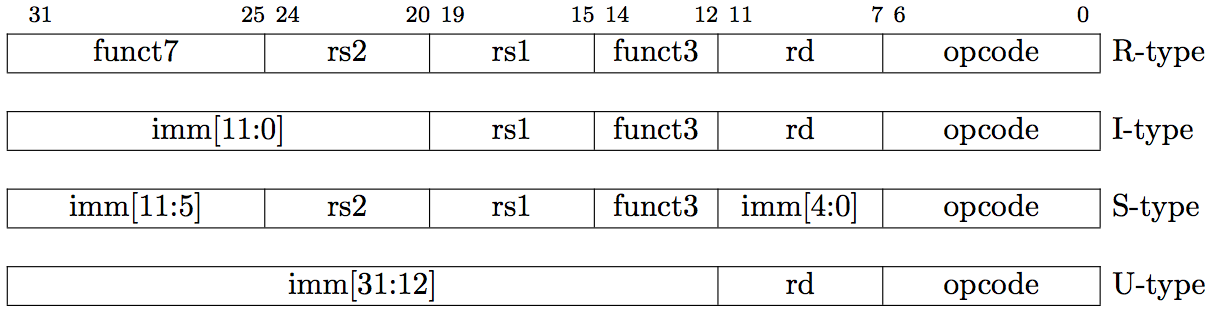
\includegraphics[width=1\textwidth]{img/instruction.png}
		\end{figure}
\end{frame}

\begin{frame}{Termos Gerais}{\textit{Load} e \textit{Store}}
	\begin{figure}
		\centering
		\label{fig:load-store}
		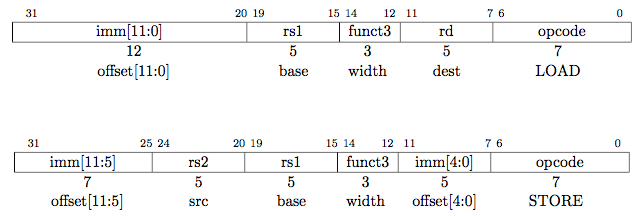
\includegraphics[width=1\textwidth]{img/load-store.png}
	\end{figure}
\end{frame}

\begin{frame}{Termos Gerais}{Exemplo de um Register-Register}
	\begin{figure}
		\centering
		\label{fig:}
		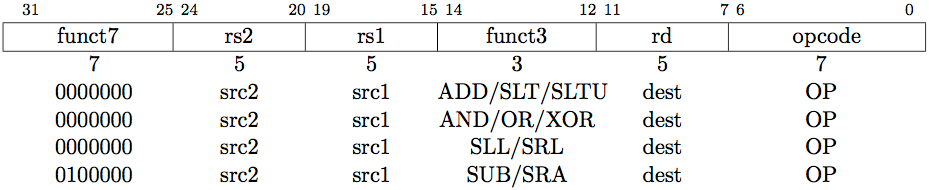
\includegraphics[width=1\textwidth]{img/register-register.png}
	\end{figure}
	\begin{itemize}
		\item \textbf{Opcode:} Local onde fica a operação principal;
		\item \textbf{Funct3:} Especificação da operação;
		\item \textbf{Funct7:} Especificação da operação;
	\end{itemize}
\end{frame}

\begin{frame}{Termos Gerais}{Demais Instruções \textit{Load} e \textit{Store}}
	\begin{figure}
		\centering
		\label{fig:real}
		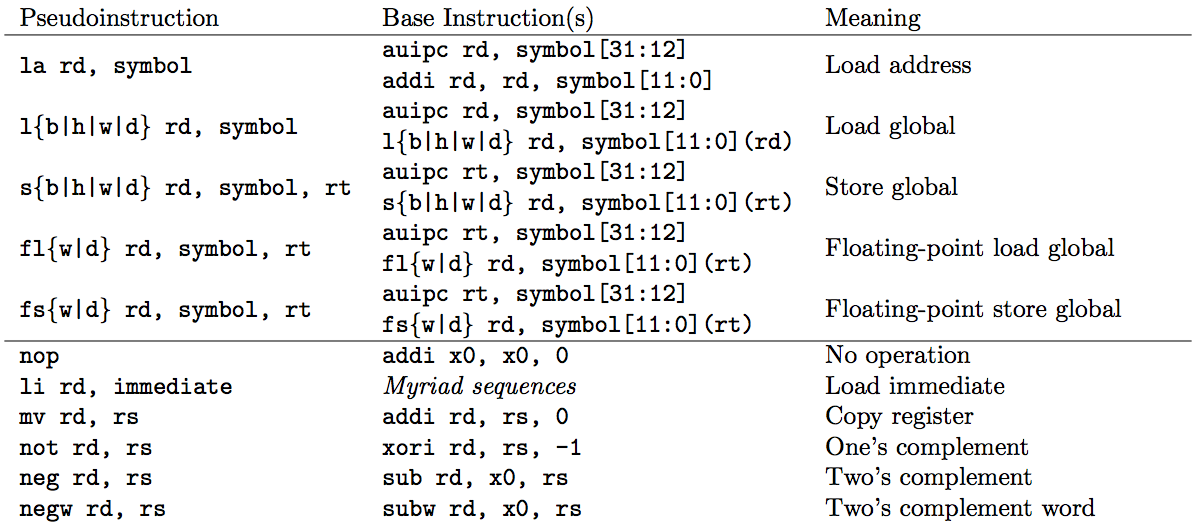
\includegraphics[width=1\textwidth]{img/real.png}
	\end{figure}
\end{frame}

\begin{frame}{Termos Gerais}{Diferenças}
	\begin{itemize}
		\setlength{\itemsep}{1.2em}
		\item RISC-V, \textbf{intencionalmente}, \textbf{não possui}:
		
		\begin{itemize}
			\item \textbf{Bit de \textit{carry}} em algumas operações aritméticas
			\begin{itemize}
				\item Não possui \textit{carry} de operações aritméticas complicadas (multiplicação e divisão);
				\item Não tem detector ou \textit{flag} para erros aritméticos, incluindo \textit{overflow}, \textit{underflow} e divisão por 0.
			\end{itemize}
			
			\item Vários Condicionais
			\begin{itemize}
				\item utiliza o \texttt{jal} (\textit{jump and link}) que armazena o endereço em um registrador para o retorno.
			\end{itemize}
		\end{itemize}
		
		\item Os projetistas dizem afirmam que isso pode simplificar o desenvolvimento do CPU, minimizando interações entre instruções;

	\end{itemize}
\end{frame}



\section{ISA Modular}

\begin{frame}{Modulação}
	\begin{itemize}
		\setlength{\itemsep}{1.5em}
		\item Por causa do crescente interesse em aceleração em processamento, a  \textbf{extensibilidade} do RISC-V é parte essencial da sua \textbf{universalidade}
		\begin{itemize}
			\setlength{\itemsep}{1em}
			\item \textbf{Pode-se adicionar módulos}, criando uma arquitetura que atende a todos os projetos de \textit{hardware}.
		\end{itemize}
		
		\item Para ativar as extensões, porções do espaço de codificação de instruções já foram reservados para uso futuro
		\begin{itemize}
			\item Ou seja, é só adicionar a nova extensão e usar.
		\end{itemize}
	\end{itemize}
\end{frame}
\begin{frame}
	\begin{figure}
		\centering
		\label{fig:bi}
		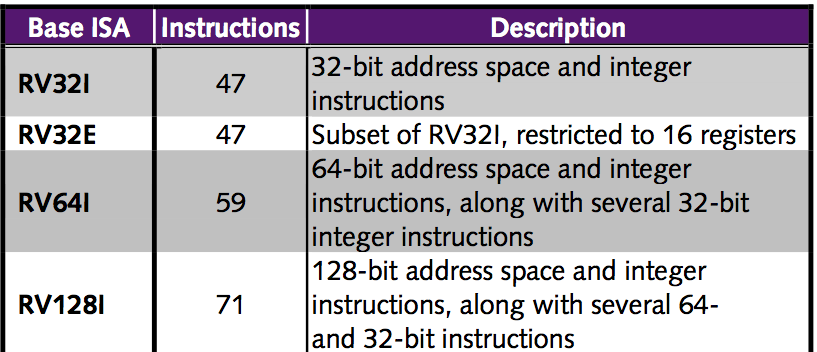
\includegraphics[width=0.9\textwidth]{img/base-instruction-a.png}
	\end{figure}
\end{frame}

\begin{frame}
	\begin{figure}
		\centering
		\label{fig:bi}
		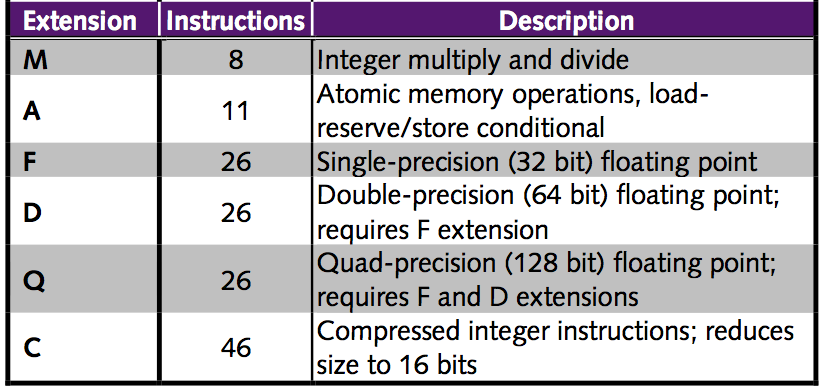
\includegraphics[width=0.9\textwidth]{img/base-instruction-b.png}
	\end{figure}
\end{frame}

\begin{frame}[plain]%{Instruções}
	\begin{figure}
		\centering
		\label{fig:bi2}
		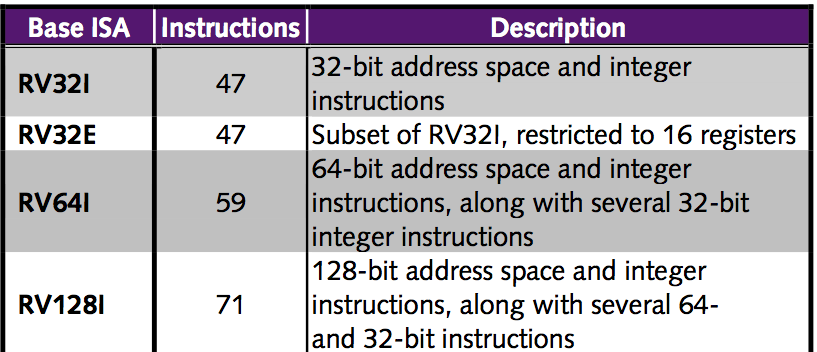
\includegraphics[width=0.7\textwidth]{img/base-instruction-a.png}
	\end{figure}
	\begin{itemize}
		\item O modelo de programação \textbf{RV32I} é escasso.
		\begin{itemize}
			\item \textit{Program Counter} e 32 registradores inteiros (\texttt{x0} - \texttt{x31}).
			\item Não contém registrador de retorno, sendo este o \texttt{x1}.
		\end{itemize}
		\item Várias combinações de imediatos, operandos e outra especificações
		\begin{itemize}
			\item O \texttt{opcode} e operando ficam em locais fixos, facilitando o processo de decodificação.
		\end{itemize}
		\item As outras bases não alteram nada.
	\end{itemize}
\end{frame}

\begin{frame}{Modelo de Memória}
	\begin{itemize}
		\setlength{\itemsep}{1.5em}
		\item Sua memória é endereçada por \textit{byte} e utiliza-se \textit{little-endian}\footnote{\textit{You store the \textbf{least} significant byte in the smallest address.}}.
		\item Enquanto outros processadores utilizam complexas instruções e vários modos de endereçamento, RISC-V usa somente \textit{base}+\textit{offset}.
		\item Podem operar em dados de tamanho 8 (\textit{byte}), 16 (\textit{half-word}), 32 (\textit{word}) ou 64 (\textit{double}) bits além das opções de sinalização.
	\end{itemize}
\end{frame}

\section{Variantes e Extensões}
\begin{frame}{Variantes e Extensões do RISC-V}{Variantes: RV32I, RV32E, RV64I e RV128I}
	\begin{itemize}
		\setlength{\itemsep}{0.5em}
		\item Todas as variantes do RISC-V descritas a seguir são baseadas do \textbf{RV32I} (já explicado).

		\bigskip

		\item \textbf{RV32E}:
		\begin{itemize}
			\item Satisfatório para implementações de \textbf{pequeno porte}. 
			
			\item Sendo um projeto menor, ocupa-se uma pequena porção de área \textit{die} e com isso
			\begin{itemize}
				\item Aumenta o custo/benefício de produção de chips;
				\item Melhora a dissipação de calor por se tratar de um chip com menos área de circuito;
			\end{itemize}
		\end{itemize}
	\end{itemize}
	\begin{block}{Resumindo}
		Redução de 32 registradores para somente o \textit{Program Counter} e \texttt{x0} - \texttt{x15}.
	\end{block}
\end{frame}

\begin{frame}{Variantes e Extensões do RISC-V}{Variantes: RV32I, RV32E, RV64I e RV128I}
	\textbf{RV64I} e \textbf{RV128I}:
	\begin{itemize}
		\setlength{\itemsep}{0.5em}
		
	
		\item Simples extensões de 64 e 128 bits.
		\item Diferença
		\begin{itemize}
			\item Aumentam o espaço de endereço e;
			\item Estende os registradores de 32 para o tamanho apropriado.
		\end{itemize}
	
		\item Essa extensão introduz novas instruções que operam com dados menores como 32 e 64 bits, de acordo com a base.
	\end{itemize}
\end{frame}

\begin{frame}%{Variantes e Extensões do RISC-V}{Extensão: Multiplicação}
		\begin{figure}
			\centering
			\label{fig:bi2}
			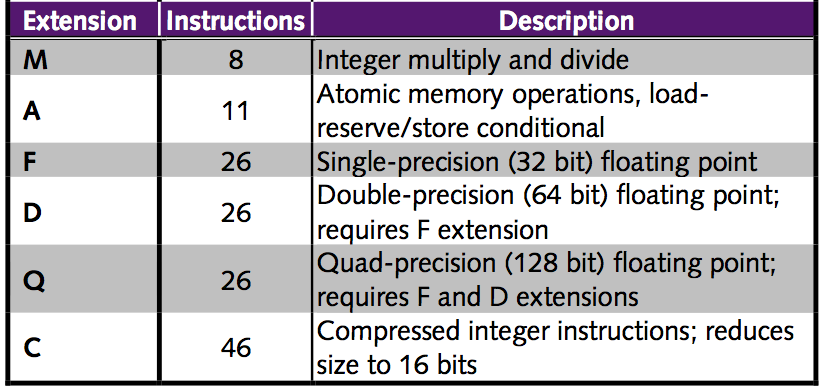
\includegraphics[width=0.7\textwidth]{img/base-instruction-b.png}
		\end{figure}
	
	\begin{itemize}
		\item \textbf{Multiplicação M}:
		\begin{itemize}
			\item Adiciona 4 instruções de multiplicação, duas de divisão, e duas de manipulação de restos.
			\item A base é indicada pela base do ISA.
			\item A divisão por 0, por exemplo, não causa interrupção, mantendo a simplicidade.
		\end{itemize}
	\end{itemize}
\end{frame}

\begin{frame}%{Variantes e Extensões do RISC-V}{Extensão: Sincronização}
	\begin{figure}
		\centering
		\label{fig:bi2}
		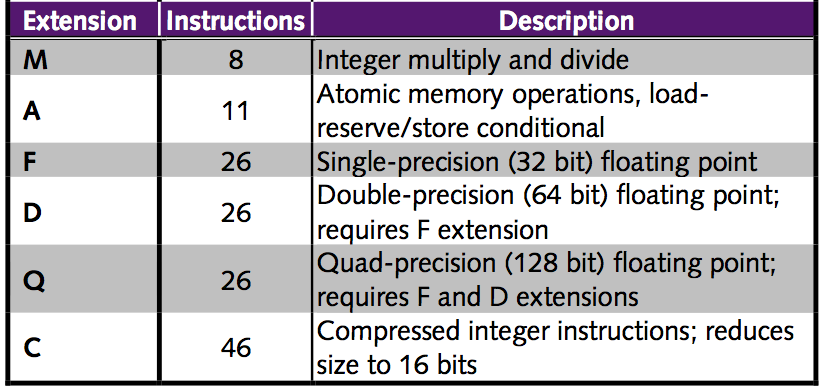
\includegraphics[width=0.7\textwidth]{img/base-instruction-b.png}
	\end{figure}
	\begin{itemize}
		\item \textbf{Sincronização A}:
		\begin{itemize}
			\setlength{\itemsep}{1.5em}
			\item Adiciona 11 instruções de sincronização visando consistência e atomicidade da operação.
			\item São divididos em dois grupos: \textit{Load} Reserved e \textit{Store} Conditional para operações atômicas na memória.
		\end{itemize}

	\end{itemize}
\end{frame}

\begin{frame}%{Variantes e Extensões do RISC-V}{Extensão: Ponto Flutuante}
	\begin{columns}
		\begin{column}{0.62\textwidth}
			\begin{figure}
				\centering
				\label{fig:bi2}
				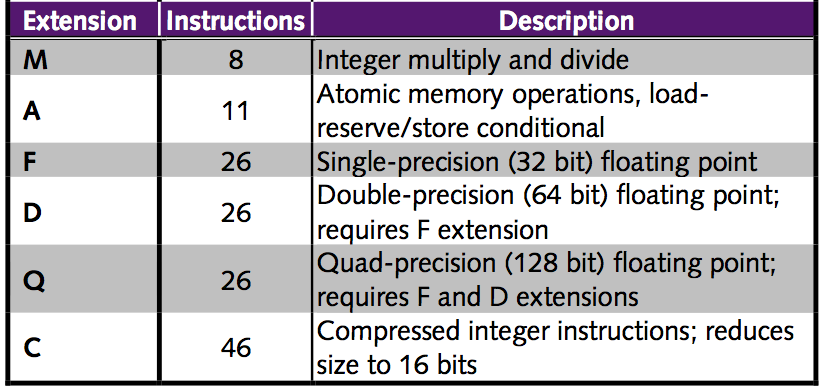
\includegraphics[width=1\textwidth]{img/base-instruction-b.png}
			\end{figure}
		\end{column}
		\begin{column}{0.4\textwidth}

			\begin{itemize}
				\setlength{\itemsep}{1.5em}
				\item Precisão simples (\textbf{F}), Precisão Dupla (\textbf{D}) e quádrupla precisão (\textbf{Q})
				\begin{itemize}
					\item Uma é pré-requisito de outra.
				\end{itemize}
			
				\item Introduz também 32 regs. de ponto flutuante (\texttt{f0} - \texttt{f31}) de 32 bits.
				\item Registrador de 5 bits para exceções
				\begin{itemize}
					\item Exceções não geram interrupções. 
				\end{itemize}
				\item As instruções \textit{load}-\textit{store} usam o mesmo endereçamento \textit{base}+\textit{offset}.
			\end{itemize}
		\end{column}
	\end{columns}
\end{frame}

\begin{frame}%{Variantes e Extensões do RISC-V}{Extensão: Compressão de Tamanho de Código}
	\begin{figure}
		\centering
		\label{fig:bi2}
		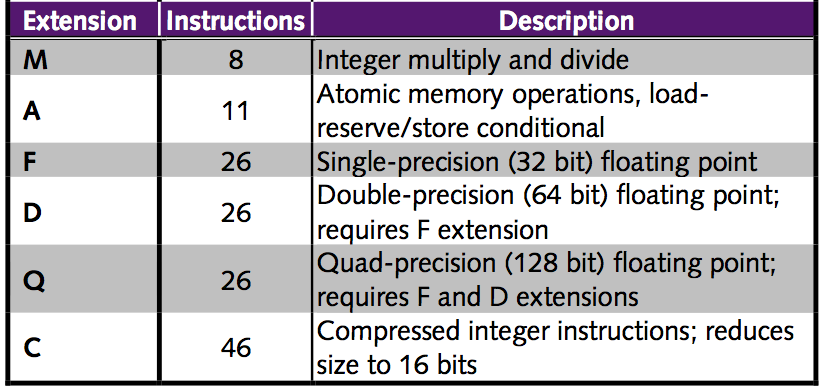
\includegraphics[width=0.6\textwidth]{img/base-instruction-b.png}
	\end{figure}
	\begin{itemize}
		\item Não adiciona nenhum outra função. Ao invés disso, \textbf{codifica} as instruções inteiras para \textbf{salvar espaço} e com isso reduzir o tamanho do \textit{footprint}.
		
		\item É disponível para bases inteiras.%, bem como \textit{load} e \textit{store} para pontos flutuantes.
		
		\item Cria-se instruções compressadas em 16 bit
		\begin{itemize}
			\item Basicamente, cada função compactada é mapeada diretamente à instrução real.
		\end{itemize}
	
		\item Visa sistemas embarcados.
	
	\end{itemize}
\end{frame}

\begin{frame}{Vantagens}
	\begin{itemize}
		\item Resumindo:
		\begin{itemize}
			\setlength{\itemsep}{1.7em}
			\item Sua área \textit{die} é menor;
			\item Permite a adição de extensões customizadas.
			\item É um projeto \textit{open-source}.
		\end{itemize}
	\end{itemize}
\end{frame}

\section{RISC-V e Linux}
\begin{frame}{\textit{Hardware} + \textit{Software}}
	\begin{itemize}
		\setlength{\itemsep}{1.7em}
		\item Um \textbf{Linux} 4.1 foi portado para o projeto RISC-V
		\begin{itemize}
			\item E um Linux Embarcado (\textbf{Yocto}) também foi disponibilizado.
		\end{itemize}
	
		\item Várias ferramentas do RISC-V incluem \textbf{compiladores} GCC, LLVM e Clang, GDB, uma suite de \textbf{verificação} e \textbf{simuladores}.

		%\item Sendo assim, ele oferece todos os recursos básicos de um RISC com implementações simplificadas, reduzindo a \textit{die area} e potencialmente, energia consumida por ele.
		
	\end{itemize}
\end{frame}

\section{Adotantes do Projeto}

\begin{frame}{Adotantes do Projeto}
	\begin{itemize}
		\setlength{\itemsep}{1.5em}
		\item Um número de organizações comerciais planejam suportar o RISC-V Foundation
		\begin{itemize}
			\setlength{\itemsep}{1em}
			\item Bluespec, Inc.;
			\item \textbf{Google};
			\item Hewlett Packard Enterprise (\textbf{HP});
			\item \textbf{Lattice} Semiconductor;
			\item Mellanox Technologies;
			\item Microsemi;
			\item \textbf{Oracle}; e
			\item Rambus Cryptography Research.
		\end{itemize}
	\end{itemize}
\end{frame}

\begin{frame}{Adotantes do Projeto}
	\begin{itemize}
		\setlength{\itemsep}{1.5em}

		\item O Instituto Indiano de Tecnologia Madras estão \textbf{desenvolvendo 6 RISC-V} \textit{open-source} para 6 tipos de usuários diferentes.
		\begin{itemize}
			\item De um pequeno CPU 32 bit para IoT até largos computadores de 64 bit concebido para computadores em escala de de armazenamento.
		\end{itemize}

		\item lowRISC é um projeto sem fins lucrativos que visa \textbf{implementar um sistema \textit{open-source} num \textit{System on Chip} (SoC)} baseado num RISC-V de 64 bits.

		\item O Laboratório de Computação, na Universidade de Cambridge, em colaboração com o FreeBSD Project, tem suportado o sistema operacional \textbf{FreeBSD para o RISC-V} 64-bit.
	\end{itemize}
\end{frame}

\begin{frame}{Adotantes do Projeto}
	\begin{itemize}
		\setlength{\itemsep}{1.5em}

		\item ETH Zurich e a Universidade de Bologna têm desenvolvido em cooperação um \textbf{System on Chip (SoC) de baixa energia} usando RISC-V.

		\item Um dos fundadores do Adapteva planeja usar \textbf{RISC-V como sucessor para o seu produto acelerador multicore}.

		\item Nvidia planeja \textbf{usá-lo} para substituir a linha de processadores Falcon \textbf{em suas placas gráficas GeForce}.
	\end{itemize}
\end{frame}


\begin{frame}[plain]
	\begin{columns}
		\begin{column}{0.48\textwidth}
			\begin{figure}
				\centering
				\label{fig:samsung2}
				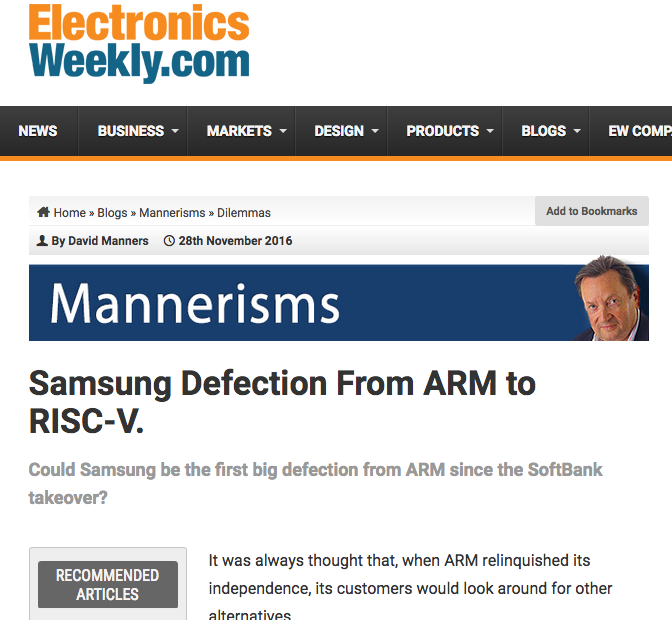
\includegraphics[width=1.05\textwidth]{img/samsung.png}
			\end{figure}
		\end{column}
		\begin{column}{0.5\textwidth}
			\pause
			\begin{itemize}
				\setlength{\itemsep}{1em}
				\item Porque continuar utilizando uma produto de uma empresa fechada como a ARM sendo que RISC-V é \textbf{independente}, \textbf{\textit{open-source}} e de \textbf{direitos livres}?
				
				\pause

				\item \textbf{Problema:} É quase impossível substituir uma arquitetura de processador em uma grande área de produto.
				\pause
				\begin{itemize}
					\item No momento não há arquitetura de processador em IoT.
				\end{itemize}

				\bigskip

				\item Nvidia e Qualcomm já estão usando RISC-V no desenvolvimento de controladores de memória GPU e processadores IoT.
			\end{itemize}
		\end{column}
	\end{columns}
\end{frame}

\begin{frame}{Dúvidas, Sugestões ou Reclamações?}
	\begin{itemize}
		\item \url{rodolfolabiapari@decom.ufop.br} \\[1cm]
		\item \url{https://www.guerrillamail.com/}
	\end{itemize}
\end{frame}

\frame{\titlepage}

\end{document}
